% https://tex.stackexchange.com/a/338201/173708
\documentclass[a4paper,portrait]{article}

\usepackage{tikz}
\usepackage[margin=0.3in]{geometry}

\usetikzlibrary{scopes}
\usetikzlibrary{intersections}
\usetikzlibrary{calc}
\usetikzlibrary{arrows.meta}

\begin{document}

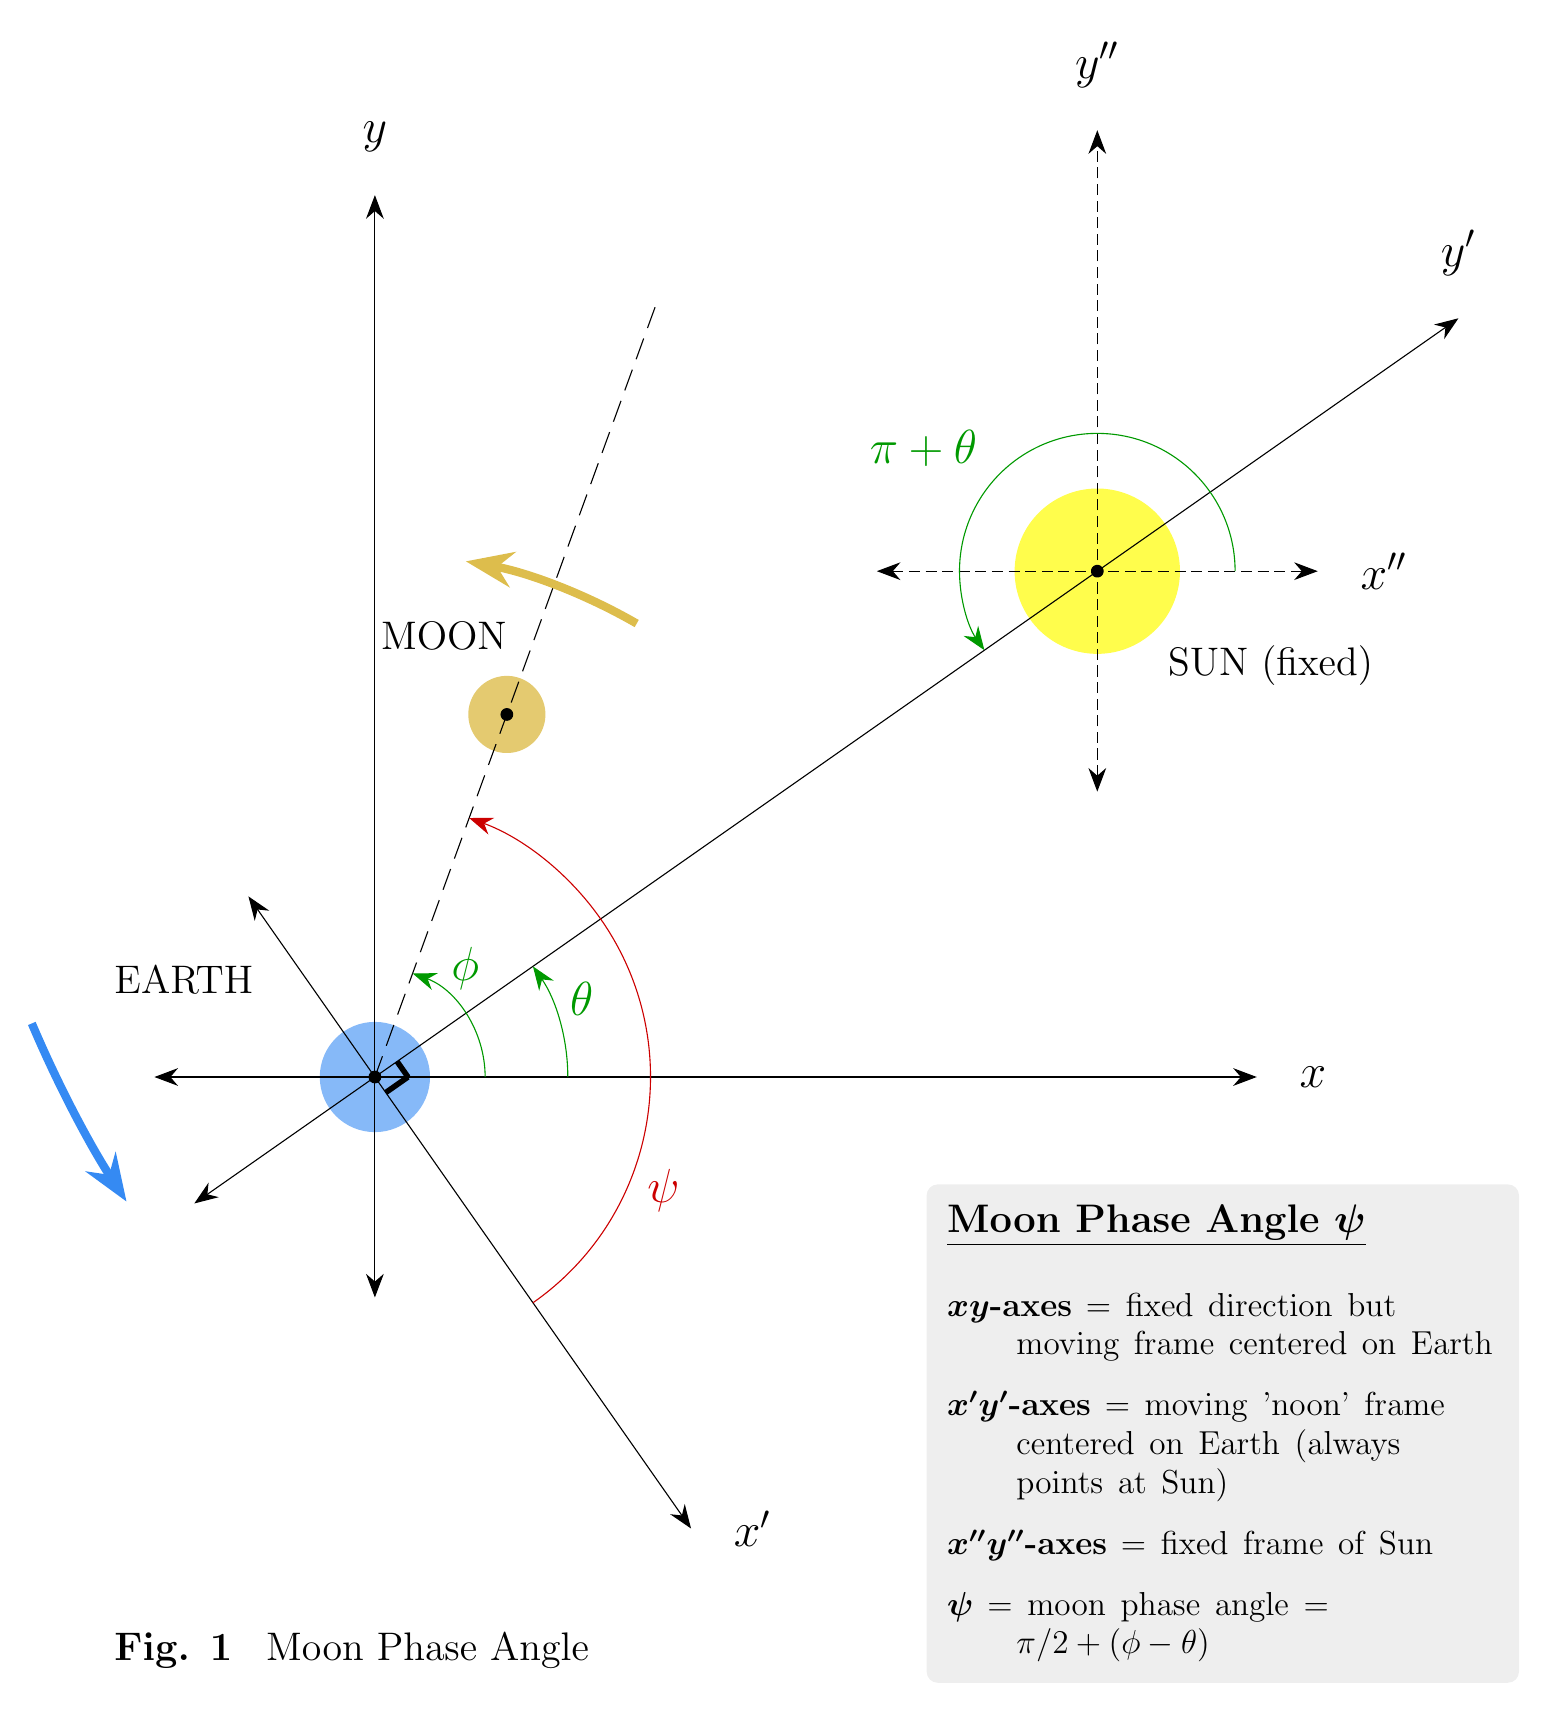
\begin{tikzpicture} [
    scale=0.7,
    node font=\LARGE,
    dashed axis/.style={dash pattern=on 4pt off 2pt},
    moon line/.style={dash pattern=on 8pt off 4pt},
    information text/.style={rounded corners, fill=Info Color, inner sep=1ex}
]

\definecolor{Earth Color}{HTML}{358af3};
\definecolor{Sun Color}{HTML}{fffc00};
\definecolor{Moon Color}{HTML}{ddbd4c};
\definecolor{Info Color}{HTML}{eeeeee};

\def\SunPosition{16};

% draw Earth xy-frame (fixed direction Earth frame), and the Earth at the origin
\fill (0, 0) [Earth Color, opacity=.6] circle (1cm);
\draw[{Stealth[length=0.3cm]}-{Stealth[length=0.3cm]}] (-4, 0) -- (16, 0) node [right=1em] {$x$};
\draw[{Stealth[length=0.3cm]}-{Stealth[length=0.3cm]}] (0, -4) -- (0, 16) node [above=1em] {$y$};
\filldraw (0, 0) circle (3pt);
\path (0, 0) node [shift={(-3.5, 1.6)}, anchor=north west] {\Large EARTH};

% draw Earth x'y'-frame (Earth frame directed at Sun, ie 'Noon-frame'), and the Sun on the y'-axis
\begin{scope}[rotate around={-55:(0, 0)}]
\fill (0, \SunPosition) coordinate (S) [Sun Color, opacity=.7] circle (1.5cm);
\draw[{Stealth[length=0.3cm]}-{Stealth[length=0.3cm]}] (-4, 0) -- (10, 0) coordinate (X') node [right=1em] {$x'$};
\draw[{Stealth[length=0.3cm]}-{Stealth[length=0.3cm]}] (0, -4) -- (0, 24) node [above=1em] {$y'$};
\filldraw (0, \SunPosition) circle (3pt);
\end{scope}
\draw[line width=2pt] (0.6,0) -- ($(0,0)!(0.6,0)!(S)$);
\draw[line width=2pt] (0.6,0) -- ($(0,0)!(0.6,0)!(X')$);

% draw arrow for Earth's orbital motion
\draw[-{Stealth[length=0.6cm]},line width=3pt,Earth Color,rotate around={203:(S)}] ($(S) + (21,0)$) arc [start angle=0, end angle=10, radius=21];

% draw Sun's x''y''-frame (fixed direction Sun frame)
\begin{scope}[shift={(S)}]
\draw[{Stealth[length=0.3cm]}-{Stealth[length=0.3cm]}, dashed axis] (-4, 0) -- (4, 0) node [right=1em] {$x''$};
\draw[{Stealth[length=0.3cm]}-{Stealth[length=0.3cm]}, dashed axis] (0, -4) -- (0, 8) node [above=1em] {$y''$};
\draw[-{Stealth[length=0.3cm]}, green!60!black] (2.5, 0) arc [start angle=0, end angle=215, radius=2.5] node[pos=0.65,above left] {$\pi + \theta$};
\path (0, 0) node [shift={(2.2,-1.2)}] {\Large SUN (fixed)};
\end{scope}

% draw Moon
\begin{scope}[rotate around={-20:(0, 0)}]
\fill (0, 7) coordinate (M) [Moon Color, opacity=.8] circle (.7cm);
\draw[moon line] (0, 0) -- (0, 15);
\filldraw (0, 7) circle (3pt);
\node [shift={(-0.8,1)}] at (0, 7) {\Large MOON};
\draw[-{Stealth[length=0.6cm]},line width=3pt,Moon Color,rotate around={-10:(0, 0)}] (0, 9.5) arc [start angle=90, end angle=110, radius=9.5];
\end{scope}

% draw various angles including Moon phase angle psi
\draw[-{Stealth[length=0.3cm]},green!60!black] (2, 0) arc [start angle=0, end angle=70, radius=2] node[pos=0.7,above right=-4pt] {$\phi$};
\draw[-{Stealth[length=0.3cm]},green!60!black] (3.5, 0) arc [start angle=0, end angle=35, radius=3.5] node[pos=0.45,above right=-2pt] {$\theta$};
\draw[-{Stealth[length=0.3cm]}, red!80!black,rotate around={-55:(0, 0)}] (5, 0) arc [start angle=0, end angle=125, radius=5] node[pos=0.3, below right=-2pt] {$\psi$};

% draw information box
\draw[shift={(10, -11)}] node[above right, text width=7cm,information text] {
    \Large
    {\boldmath
    \textbf{\underline{Moon Phase Angle $\psi$}} }

    \vspace{1ex}
    \large
    \begin{description}
    {\boldmath
    \item[$xy$-axes]= fixed direction but moving frame centered on Earth
    \item[$x'y'$-axes]= moving 'noon' frame centered on Earth (always points at Sun)
    \item[$x''y''$-axes]= fixed frame of Sun
    \item[$\psi$]= moon phase angle =} $\pi/2 + (\phi - \theta)$
    \end{description}
};

\node[above right] at (-5, -11) {\Large \textbf{Fig. 1} \hspace{0.1cm} Moon Phase Angle};

\end{tikzpicture}

\end{document}
